\clearpage
\title{Implementing Interpolation; Newton's Forward Method in MATLAB }
\author{}
\date{}
\maketitle

\section*{Introduction}
\subsection*{Interpolation, Newton's Forward Method}
Newton's Forward Interpolation is a numerical technique used for interpolating or estimating the value of a function between given data points. It belongs to the category of polynomial interpolation methods and is particularly useful when dealing with equally spaced data points.
\\\\
The method involves constructing a polynomial of degree \(n\) that passes through \(n+1\) equally spaced data points. It approximates the value of the function at an intermediate point within the range of the given data.
The general form of the Newton's Forward Interpolation polynomial is:
\[f(x) = P_n(x) = f(x_0) + \Delta y_0 \cdot P_1(u) + \Delta^2 y_0 \cdot P_2(u) + \ldots\]
Here, \(P_n(x)\) is the polynomial of degree \(n\) used for interpolation, \(f(x_0)\) represents the value of the function at the starting point \(x_0\), \(\Delta y_0\) denotes the first forward difference, \(\Delta^2 y_0\) signifies the second forward difference, and so on. The symbol \(u\) typically represents the normalized difference ratio \(\frac{x - x_0}{h}\), where \(h\) is the common difference between the data points.\\\\


\section*{Tools Used}
\begin{itemize}
    \item MATLAB R2021a - for writing and running code.
    \item MacTeX -\LaTeX  compiler.
    \item VS Code with \LaTeX workshop extension as a text editor.
\end{itemize}

\section*{Process}

\subsection*{Code for Newton's Forward Interpolation:}
\begin{minted}[breaklines, linenos]{matlab}

\end{minted}

\subsection*{Output}
\begin{center}
    \centering
    % 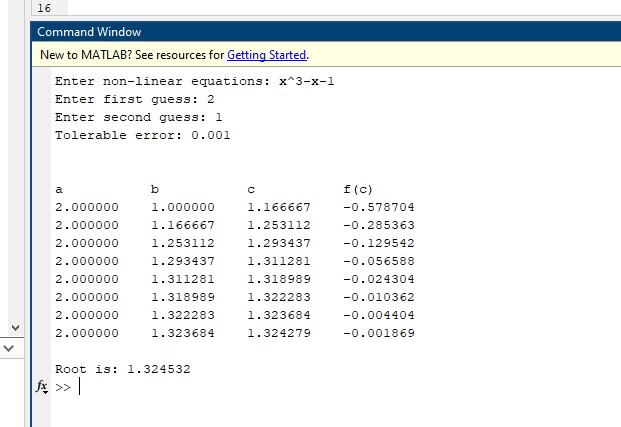
\includegraphics[width = .9\textwidth]{false.jpeg}
    \captionof{figure}{Newton's Forward Method}
\end{center}